Pavel has a toy railway. It is very simple. There is a single main line consisting of $n$ stations. These stations are numbered from $0$ to $n - 1$ in order along the line. The distance between the stations $i$ and $i + 1$ is $l_i$ centimeters ($0 \leq i < n - 1$).

Apart from the main line there may be some secondary lines. Each secondary line is a railway line between a station on the main line and a new station that does not lie on the main line. (These new stations are not numbered.) At most one secondary line can start in each station of the main line. The length of the secondary line starting at station $i$ is $d_i$ centimeters. We use $d_i = 0$ to denote that there is no secondary line starting at station $i$.

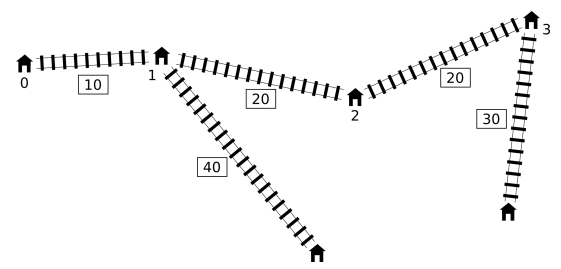
\includegraphics[scale=0.9]{1.png}

Pavel is now planning to build one shortcut: an express line between two different (possibly neighbouring) stations of \textbf{the main line}. Express line will have length of exactly $c$ centimeters, regardless of what two stations it will connect.

Each segment of the railway, including the new express line, can be used in both directions. The \textbf{distance} between two stations is the smallest length of a route that goes from one station to the other along the railways. The \textbf{diameter} of the whole railway network is the maximum distance among all pairs of stations. In other words, this is the smallest number $t$, such that the distance between every pair of stations is at most $t$.

Pavel wants to build the express line in such a way that the diameter of the resulting network is minimized.

\textbf{Implementation details}

You should implement the function
\texttt{int64 find\_shortcut(int n, int[] l, int[] d, int c) }

\begin{itemize}
\item \texttt{n}: number of stations on the main line,
\item \texttt{l}: distances between stations on the main line (array of length $n - 1$),  
\item \texttt{d}: lengths of secondary lines (array of length $n$),
\item \texttt{c}: length of the new express line.
\item the function should return the smallest possible diameter of the railway network after adding the express line.
\end{itemize}


